\documentclass[a4paper, 12pt]{report}


\usepackage[english]{babel}
\usepackage[utf8]{inputenc}
\usepackage{graphicx}
\usepackage[a4paper, width=150mm, top=25mm, bottom=25mm]{geometry}
\usepackage{mathptmx}
\usepackage[T1]{fontenc}
\usepackage{enumitem}
\usepackage{amsmath}
\usepackage{index}
\usepackage{fancyhdr}
\usepackage{titlesec}
\usepackage{subfig}
\usepackage{listings}
\usepackage{listings-rust}
\titleformat{\chapter}{\normalfont\huge}{\thechapter.}{20pt}{\huge\it}

\graphicspath{ {images/} }
\makeindex

\usepackage{listings}
\usepackage{xcolor}

\definecolor{codegreen}{rgb}{0,0.6,0}
\definecolor{codegray}{rgb}{0.5,0.5,0.5}
\definecolor{codepurple}{rgb}{0.58,0,0.82}
\definecolor{backcolour}{rgb}{0.95,0.95,0.92}

\lstdefinestyle{mystyle}{
    backgroundcolor=\color{backcolour},   
    commentstyle=\color{codegreen},
    keywordstyle=\color{magenta},
    numberstyle=\tiny\color{codegray},
    stringstyle=\color{codepurple},
    basicstyle=\ttfamily\footnotesize,
    breakatwhitespace=false,         
    breaklines=true,                 
    captionpos=b,                    
    keepspaces=true,                 
    numbers=left,                    
    numbersep=5pt,                  
    showspaces=false,                
    showstringspaces=false,
    showtabs=false,                  
    tabsize=2
}


\usepackage{hyperref}
\hypersetup{
    colorlinks=true,
    linkcolor=blue,
    filecolor=magenta,      
    urlcolor=cyan,
}

\urlstyle{same}
\lstset{style=mystyle}

\begin{document}
\title{\Large{\textbf{Optimization Assignment Thing}}}
\author{Henning W.}
\date{14/04/2021}
\maketitle
\tableofcontents
\setcounter{page}{2}
\fancyhf{}
\renewcommand{\headrulewidth}{2pt}
\renewcommand{\headrulewidth}{2pt}
\pagestyle{fancy} % Turn on the style
\fancyhf{} % Start with clearing everything in the header and footer
% Set the right side of the footer to be the page number
\fancyfoot[R]{\thepage}

% Redefine plain style, which is used for titlepage and chapter beginnings
% From https://tex.stackexchange.com/a/30230/828
\fancypagestyle{plain}{%
    \renewcommand{\headrulewidth}{0pt}%
    \fancyhf{}%
    \fancyfoot[R]{\thepage}%
}

\chapter{Acknowledgements}
This paper is written by a student, on a subject in which he is not comfortable in saying, that he has THE best solution to. Especially because said student(me), also knows that there are many more enhancements that can be done to the project.

I would also like to the clarify, that the optimized version of this program has been modified in more ways than just speed. An example of this is retrieval of the absolute path of a resource, instead of a hard coded path to the resource. The code has been modified further, however, to make an attempt at making the code more readable. In hindsight, this could be considered a violation, considering how there could be other people working on the same code in a real life scenario. I admit, that in practice one should attempt to optimize what you're told to optimize, and nothing else. Then, if there should be any other optimizations you wish to make, then you should make a suggestion with the rest of the team (assuming there is one).

\chapter{Introduction}

This small revolves around the optimization of self-chosen project. One also had the option of choosing a project, which one of the teachers had chosen. Due to the fact, that most of my projects utilize a multitude of libraries, in which the logic is implemented inside said libraries, the actual potential of me personally optimizing those projects is limited. Because of this, the project "letterfrequencies", which was supplied by the teachers, has been chosen for this assignment.

This program was designed to iterate through a file, and print out the sum of each occurrence of each separate letter. 

Since an explanation of which part was to be optimized in the code, I should clarify, that most of the code has been changed in more ways, than just speed. Therefore the program will have more than a few changes. But the main changes revolves around changing the FileReader to a BufferedReader, and to limit the amount of times the program iterates through hashmaps. Disclaimer - The old Java file is not entirely pristine. This is largely due to the fact, that I had to print the csv files. 

Documentation of old and new performance can be found in old\_data.csv and data.csv respectively - Both inside the resources folder.

I didn't use any special software for determining the problems. Just my brain.

Since documentation of mean and standard deviation values were also recommended, a small python program has been created. The program converts both files into panda dataframes and utilizes their functions to find the mean and standard deviation values of both the optimized and non-optimized versions. This program can be run by the user if wanted, or a screenshot can be found in ./resources/results\_screenshot.png

\begin{figure}[ht]
\centering
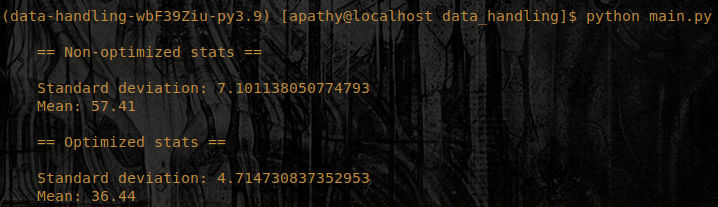
\includegraphics[width=12cm]{../resources/results_screenshot.png}
\caption{Screenshot of results}
\label{trash}
\label{praise kek}
\end{figure}

\chapter{Possible Speed Improvements}
Lets look at some of the features that can be improved.
\begin{itemize}
	\item The initial project uses longs. Longs in Java are $2^{64}$. In comparison, integers in Java are signed $2^{32}$ bits or $-2.147.483.648$ to $2.147.483.648$. The longest novel on earth is "A Chronicle of Ancient Sunlight" \footnote{{https://en.wikipedia.org/wiki/List\_of\_longest\_novels}}  with $2.436.924$ words. For it to surpass the limit of the integer data type, the average amount of letters in each word would have to be $881.22$. I.e. the Integer is more than enough.
	\item My original assessment of the speed of hashmaps versus arrays was, that hashmaps would always be slower than arrays. Turns out that that's not always the case \footnote{https://stackoverflow.com/questions/6462055/hashmap-vs-array-performance}. What can be said is, that the speed of the lookup will drastically change if the Hashmap is sorted \footnote{https://www.baeldung.com/java-hashmap} . This changes the lookup from O(n) to O(log n) via. a binary search. 
	\item There are many ways of reading a file in Java. The default one is FileReader. The optimized version I made uses BufferedReader instead. There are even faster ways of reading files, such as MappedByteBuffer\footnote{https://docs.oracle.com/javase/8/docs/api/java/nio/MappedByteBuffer.html}.
	
	
\end{itemize}
\chapter{Bottlenecks and fixes}

The largest change in speed can be explained a quote from 
\url{https://www.geeksforgeeks.org/difference-between-bufferedreader-and-filereader-in-java/}:

\begin{quote}
A buffer is a small portion of the device memory storage used to temporarily store some amount of data. Usually, Buffers use the RAM of the device to store the temporary data, and hence, accessing data from the buffer is much faster than accessing the same amount of data from the hard drive. 
\end{quote}

As such the FileReader was changed

\begin{lstlisting}[language=java]
Reader reader = new FileReader(RESOURCES_DIRECTORY+FILE_NAME);
\end{lstlisting}

To

\begin{lstlisting}[language=java]
private static BufferedReader getFileFromResources(String fileName) throws FileNotFoundException {
		return new BufferedReader(new FileReader(RESOURCES_DIRECTORY + fileName));
}
\end{lstlisting}

Largest change code wise was deleting this method entirely:

\begin{lstlisting}[language=java]
private static void print_tally(Map<Integer, Long> freq) {
        int dist = 'a' - 'A';
        Map<Character, Long> upperAndlower = new LinkedHashMap();
        for (Character c = 'A'; c <= 'Z'; c++) {
            upperAndlower.put(c, freq.getOrDefault(c, 0L) 
            + freq.getOrDefault(c + dist, 0L));
        }
        Map<Character, Long> sorted = upperAndlower.entrySet()
        				.stream()
                .sorted(Collections.reverseOrder
                		(Map.Entry.comparingByValue()))
                .collect(
                		toMap(Map.Entry::getKey, Map.Entry::getValue, 
                		(e1, e2) -> 
                		e2,LinkedHashMap::new));
        for (Character c : sorted.keySet()) {
            System.out.println("" + c + ": " + sorted.get(c));
            ;
        }
    }
\end{lstlisting}
\newpage
And changing this method:

\begin{lstlisting}[language=java]
 private static void tallyChars(Reader reader, Map<Integer, Long> freq) throws IOException {
        int b;
        while ((b = reader.read()) != -1) {
            try {
                freq.put(b, freq.get(b) + 1);
            } catch (NullPointerException np) {
                freq.put(b, 1L);
            }
            ;
        }
    }

\end{lstlisting}

To this:
\begin{lstlisting}[language=java]
    private static Map<Character, Integer> createMapOfCharacters
    (Reader reader) throws IOException {
        Map<Character, Integer> mapOfCharacters = new HashMap<>();
        int b;
        while ((b = reader.read()) != -1) {
            Character letter = Character.toUpperCase((char) b);
            if (letter >= 'A' && letter <= 'Z')
                if (mapOfCharacters.containsKey(letter)) {
                    mapOfCharacters.put
                    (letter, mapOfCharacters.get(letter) + 1);
                } else {
                    mapOfCharacters.put(letter, 0);
                }
        }
        return mapOfCharacters;
    }
\end{lstlisting}

This means, that the program no longer populates the hashmap with values and then iterates through it to reverse the order and collects it in a new hashmap. Instead it just puts the values in in the correct order to begin with.

Note that we use integers instead of longs. 

Apart from that, optimizations which aren't related to speed were made. As a rule of thumb code is for humans. Because of this, all my variables and method names are self-explanatory. 

\chapter{Conclusion}
Further optimizations can be made e.g. using the MappedByteBuffer. If one was so inclined, threading could also be used (assuming that the downsides would be bearable).

\end{document}